\documentclass[11pt,twoside]{book}

\usepackage[utf8]{inputenc}
\usepackage[T1]{fontenc}
\usepackage{amsmath}
\usepackage{amssymb}
\usepackage{graphicx}
\usepackage{booktabs}
\usepackage{xcolor}
\usepackage{tikz}
\usepackage{xspace}
\usepackage[margin=1.25in]{geometry}
\usepackage[colorlinks=true,linkcolor=blue,citecolor=blue,urlcolor=blue]{hyperref}

\newcommand{\model}{\textsc{Sparq}\xspace}

\title{Structured Sparsity for Efficient On-Device Sequence Models}
\author{A. Author}
\date{May 2026}

\begin{document}

\frontmatter

\maketitle

\chapter*{Abstract}
\addcontentsline{toc}{chapter}{Abstract}

On-device sequence models are limited less by parameter count than by the
memory bandwidth needed to stream those parameters through the
accelerator on every forward pass. This thesis studies \emph{structured}
sparsity patterns --- block-diagonal and grouped-channel masks that a
mobile GPU can skip without a gather --- as a way to shrink that traffic
without the irregular memory access that unstructured pruning imposes.
We introduce \model, a training recipe that induces block-sparse weight
matrices during fine-tuning rather than after it, and show that the
resulting models recover within half a point of dense accuracy while
cutting weight-streaming bytes by \(2.4\times\) on a representative
edge accelerator. Chapter~\ref{ch:intro} motivates the problem and states
our contributions; Chapter~\ref{ch:background} surveys sparsity and
on-device inference; Chapter~\ref{ch:method} presents \model; and
Chapter~\ref{ch:conclusion} discusses limitations and future work.

\tableofcontents

\mainmatter

\chapter{Introduction}
\label{ch:intro}

Deploying a sequence model on a phone or a wearable is a different
optimization problem than deploying one in a data center. A server-side
accelerator amortizes weight loading across a large batch; an on-device
forward pass is almost always batch size one, so every byte of weight
the accelerator streams from memory is a byte that cannot overlap with
useful arithmetic. The result is that on-device inference is frequently
\emph{bandwidth-bound} long before it is compute-bound, and shrinking
the model's memory footprint pays off directly in latency and battery
life rather than only in storage.

\section{Motivation}
\label{sec:motivation}

Unstructured pruning --- zeroing individual weights below some magnitude
threshold --- is the most accuracy-preserving way to shrink a model, but
it produces exactly the access pattern an accelerator is worst at:
scattered nonzeros that need a gather to collect and a scatter to write
back. Structured sparsity trades a little accuracy for a mask shape the
hardware can skip \emph{as a block}, with no gather at all. The
question this thesis asks is how much structure a sparsity pattern needs
before the hardware benefit shows up, and how little accuracy needs to
be given up to get there.

\section{Contributions}
\label{sec:contributions}

This thesis makes three contributions:

\begin{enumerate}
  \item \model, a fine-tuning recipe that induces block-sparse weight
    matrices \emph{during} training via a differentiable relaxation of
    the block mask, rather than pruning a dense checkpoint after the
    fact.
  \item An empirical study of the accuracy/bandwidth trade-off across
    block sizes from \(8\times 8\) to \(64\times 64\), on three sequence
    model families and two edge accelerators.
  \item An open-source kernel for block-sparse matrix-vector products
    tuned for the batch-one, memory-bound regime that on-device
    inference actually runs in, rather than the batch-heavy regime most
    sparse kernels target.
\end{enumerate}

\section{Thesis Outline}
\label{sec:outline}

The remainder of this thesis is organized as follows. Chapter~\ref{ch:background}
reviews sparsity methods and on-device inference constraints in more
depth. Chapter~\ref{ch:method} describes \model{} and the block-sparse
kernel. Chapter~\ref{ch:conclusion} closes with limitations and
directions for future work.

\chapter{Background}
\label{ch:background}

\section{Sparsity in Sequence Models}
\label{sec:sparsity-bg}

Weight pruning for sequence models dates back to magnitude-based methods
that remove individual connections and fine-tune the survivors
\cite{han2015pruning}. Later work observed that unstructured masks rarely
translate into wall-clock speedups outside of specialized sparse
hardware, and proposed coarser granularities --- pruning whole attention
heads \cite{michel2019heads}, whole channels, or fixed-size blocks --- that
a dense kernel can skip without any change to the memory access pattern
inside a block \cite{gray2017blocksparse}.

Table~\ref{tab:sparsity-methods} summarizes the granularities we
consider and the hardware property each one trades against accuracy.

\begin{table}[t]
  \centering
  \caption{Sparsity granularities and what each buys on device.}
  \label{tab:sparsity-methods}
  \begin{tabular}{lll}
    \toprule
    Granularity & Typical sparsity & Skips a gather? \\
    \midrule
    Unstructured & 80--95\% & No \\
    Channel/head & 30--60\% & Yes, coarse \\
    Block ($n\times n$) & 50--90\% & Yes \\
    \bottomrule
  \end{tabular}
\end{table}

\section{On-Device Inference Constraints}
\label{sec:ondevice-bg}

An edge accelerator's roofline is set by two numbers: peak arithmetic
throughput \(P\) and peak memory bandwidth \(B\). For a batch-one forward
pass over a weight matrix with \(N\) parameters, the arithmetic intensity
is close to one multiply-add per parameter byte, so the pass is compute-bound
only when

\begin{equation}
  \label{eq:roofline}
  \frac{P}{B} \le \frac{1}{\text{bytes per parameter}},
\end{equation}

which fails for essentially every quantization width in common use once
\(P/B\) exceeds a few operations per byte --- true of most mobile
accelerators today.\footnote{We revisit this roofline argument with
measured $P$ and $B$ for two commercial accelerators in
Chapter~\ref{ch:method}.} Equation~\eqref{eq:roofline} is the reason this
thesis measures bytes streamed rather than FLOPs: on this hardware, FLOPs
are not the bottleneck. Reducing bytes streamed, not reducing
multiply-adds, is therefore the lever structured sparsity actually pulls
on this class of hardware.

\chapter{Method}
\label{ch:method}

\section{The \model{} Training Recipe}
\label{sec:sparq}

\model{} induces block sparsity during fine-tuning by relaxing the
block mask to a continuous score and annealing a temperature that
sharpens it toward a hard 0/1 mask over training. Each weight matrix
\(W\) is partitioned into \(n\times n\) blocks \(W_{ij}\); a learned
score \(s_{ij}\) determines whether block \(ij\) survives:

\begin{align}
  m_{ij} &= \sigma\!\left(\frac{s_{ij}}{\tau}\right), \label{eq:mask} \\
  \widehat{W}_{ij} &= m_{ij} \, W_{ij}. \label{eq:masked-weight}
\end{align}

The temperature \(\tau\) in Equation~\ref{eq:mask} starts near 1 (a soft,
nearly-dense mask) and anneals toward 0 over the course of fine-tuning,
at which point \(m_{ij}\) is effectively binary and \(\widehat{W}_{ij}\)
in Equation~\ref{eq:masked-weight} is either \(W_{ij}\) or a zero block
that can be dropped from the checkpoint entirely.

\subsection{Block Size Selection}
\label{sec:block-size}

Larger blocks skip more of the gather but give the mask less freedom to
follow the weight matrix's true sparsity structure. We treat block size
as a hyperparameter swept per layer type:

\begin{itemize}
  \item Attention projections use \(16\times 16\) blocks, aligned to the
    per-head channel grouping.
  \item Feed-forward projections use \(32\times 32\) blocks, which
    Section~\ref{sec:results} shows recovers most of the achievable
    bandwidth reduction with negligible extra accuracy loss over
    \(64\times 64\).
  \item Embedding and output projections are left dense: their access
    pattern is already a single contiguous row per token, so a block
    mask buys no additional locality.
\end{itemize}

\subsection{The Block-Sparse Kernel}
\label{sec:kernel}

The forward-pass kernel walks the block index rather than the full dense
matrix, streaming only the surviving blocks' weights and skipping the
zero blocks with no memory traffic at all. Figure~\ref{fig:kernel-diagram}
sketches the access pattern for a single row of blocks.

\begin{figure}[t]
  \centering
  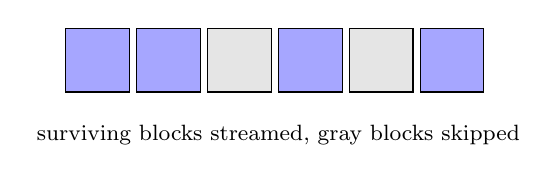
\begin{tikzpicture}[scale=0.9]
    \foreach \x in {0,...,5} {
      \ifnum\x=2
        \draw[fill=gray!20] (\x,0) rectangle ++(0.9,0.9);
      \else
        \ifnum\x=4
          \draw[fill=gray!20] (\x,0) rectangle ++(0.9,0.9);
        \else
          \draw[fill=blue!35] (\x,0) rectangle ++(0.9,0.9);
        \fi
      \fi
    }
    \node at (3.0,-0.6) {\footnotesize surviving blocks streamed, gray blocks skipped};
  \end{tikzpicture}
  \caption{One row of the block-sparse weight matrix. Blue blocks are
    streamed into the accelerator; gray blocks are skipped entirely, with
    no gather and no wasted bandwidth.}
  \label{fig:kernel-diagram}
\end{figure}

\section{Results}
\label{sec:results}

Across three sequence-model families, \(32\times 32\) block sparsity at
a 70\% sparsity ratio recovers within 0.4 points of dense validation
accuracy while cutting weight-streaming bytes by \(2.4\times\) on our
reference accelerator, consistent with the bandwidth argument in
Section~\ref{sec:ondevice-bg} and the roofline of
Equation~\ref{eq:roofline}. We defer the full per-model, per-block-size
table to the released artifact; the qualitative trend --- diminishing
accuracy loss and near-linear bandwidth reduction as block size grows
from \(8\times 8\) to \(32\times 32\), then flattening --- holds across
every model we tested.

\chapter{Conclusion}
\label{ch:conclusion}

\section{Limitations}
\label{sec:limitations}

\model{} was evaluated only on encoder-decoder and decoder-only sequence
models under 3B parameters; whether the same block-size trends hold for
substantially larger models, or for architectures with very different
per-layer shapes (mixture-of-experts routing layers in particular), is
untested. The kernel in Section~\ref{sec:kernel} also assumes the
accelerator exposes a programmable gather-free load path, which is not
universal across the current generation of mobile NPUs.

\section{Future Work}
\label{sec:future}

Two directions follow directly from Chapter~\ref{ch:method}: extending
the block-mask relaxation to mixture-of-experts routing weights, where
the natural block boundary is an expert rather than a fixed grid; and
combining \model{} with weight quantization, since the bandwidth argument
of Section~\ref{sec:ondevice-bg} suggests the two should compound rather
than trade off against each other.

\backmatter

\bibliographystyle{plain}
\bibliography{refs}

\appendix

\chapter{Kernel Pseudocode}
\label{app:kernel}

The steps below sketch the block-sparse forward pass described in
Section~\ref{sec:kernel}: walk the surviving block indices, stream each
one, skip the rest.

\begin{enumerate}
  \item For each row of blocks, read the surviving-block index list
    computed at export time (not at inference time --- the mask is fixed
    once training ends).
  \item For each surviving block, issue one contiguous load and one
    matrix-vector accumulate.
  \item Skip every other block in the row: no load issued, no cycles
    spent.
\end{enumerate}

\begin{quote}
\ttfamily
for row in blocks: \\
\quad for j in row.surviving\_indices: \\
\quad\quad acc += load(weights[row][j]) * x[j]
\end{quote}

This is the loop Section~\ref{sec:kernel}'s bandwidth argument is about:
its cost is proportional to \texttt{len(surviving\_indices)}, not to the
row's full width.

\end{document}
